% Original replacement exercises -- chapters 1 and 2 (sessions 1 to 14).
% \DefExo{session}{target}{statement}{detailed solution}{number of student answer lines}

% -----------------------------------------------------------------------------
% Chapter 1 -- Numerical sequences
% -----------------------------------------------------------------------------
\DefExo{1}{Recognise an arithmetic sequence by differences}{%
A warehouse manager is testing three models. For every natural number $n$, $n$ is the week number.
\begin{itemize}
\item Number of parcels prepared: $a_n=3(2n+7)-n$.
\item Number of customer complaints: $b_n=2n^2-n+4$.
\item Number of pallets still in stock: $c_n=150-7n$.
\end{itemize}
\begin{enumerate}[label=\alph*.]
\item For each of the three sequences, calculate $u_{n+1}-u_n$ (with $u=a$, $b$ or $c$) and state whether the sequence is arithmetic; if so, give its common difference.
\item For each arithmetic sequence, interpret the common difference in context.
\end{enumerate}
}{%
\begin{enumerate}[label=\alph*.]
\item \textbf{Sequence $(a_n)$.} Expanding: $a_n=6n+21-n=5n+21$. Then $a_{n+1}-a_n=5(n+1)+21-(5n+21)=5$. The difference is constant: $(a_n)$ is arithmetic with common difference $5$ (first term $a_0=21$).

\textbf{Sequence $(b_n)$.} $b_{n+1}-b_n=2(n+1)^2-(n+1)+4-(2n^2-n+4)=2(2n+1)-1=4n+1$. This difference depends on $n$: for example $b_0=4$, $b_1=5$, $b_2=10$, so $b_1-b_0=1$ and $b_2-b_1=5$. The sequence $(b_n)$ is not arithmetic.

\textbf{Sequence $(c_n)$.} $c_{n+1}-c_n=150-7(n+1)-(150-7n)=-7$. The sequence $(c_n)$ is arithmetic with common difference $-7$ (first term $c_0=150$).
\item Each week, the warehouse prepares $5$ more parcels than the week before. Each week, the stock goes down by $7$ pallets (a negative common difference means a decrease).
\end{enumerate}
}{4}

\DefExo{2}{General term and distant terms (arithmetic)}{%
A delivery company is gradually replacing its diesel vehicles with electric ones. At the start of 2025 (rank $0$), it owns $186$ diesel vehicles and it withdraws $4$ of them every year. Let $d_n$ be the number of diesel vehicles at the start of the year $2025+n$; the sequence $(d_n)$ is arithmetic.
\begin{enumerate}[label=\alph*.]
\item Give the first term $d_0$ and the common difference of the sequence $(d_n)$.
\item Express $d_n$ in terms of $n$ for every natural number $n$.
\item Calculate $d_{12}$ and $d_{30}$. Interpret $d_{30}$ in a sentence.
\end{enumerate}
}{%
\begin{enumerate}[label=\alph*.]
\item $d_0=186$; $4$ vehicles are withdrawn each year, so $d_{n+1}=d_n-4$: the common difference is $r=-4$.
\item For an arithmetic sequence with first term $d_0$: $d_n=d_0+nr$, that is $d_n=186-4n$.
\item $d_{12}=186-4\times12=186-48=138$ and $d_{30}=186-4\times30=186-120=66$.

Rank $30$ corresponds to the year $2025+30=2055$: according to this model, the company will still own $66$ diesel vehicles at the start of 2055.
\end{enumerate}
}{4}

\DefExo{3}{Sum of consecutive integers}{%
\begin{enumerate}[label=\alph*.]
\item Calculate $\displaystyle\sum_{i=1}^{365}i=1+2+\cdots+365$.
\item Calculate $\displaystyle\sum_{k=100}^{365}k=100+101+\cdots+365$. State the number of terms in this sum.
\item To build up some savings, Lova takes on a challenge: on the $k$-th day of the year, she puts $k$ cents into a money box ($1$ cent on day $1$, $2$ cents on day $2$, and so on). How much, in euros, will she have put in altogether over a $365$-day year? And from day $100$ to day $365$ inclusive?
\end{enumerate}
}{%
\begin{enumerate}[label=\alph*.]
\item The integers from $1$ to $365$ form an arithmetic sequence with common difference $1$; there are $365$ terms. So
$\displaystyle\sum_{i=1}^{365}i=365\times\frac{1+365}{2}=365\times183=66\,795$.
\item From $100$ to $365$ there are $365-100+1=266$ terms. So
$\displaystyle\sum_{k=100}^{365}k=266\times\frac{100+365}{2}=266\times232.5=61\,845$.

Check: $66\,795-61\,845=4\,950=\dfrac{99\times100}{2}$, which is indeed the sum of the integers from $1$ to $99$.
\item The total for the year is $66\,795$ cents, that is €$667.95$. From day $100$ to day $365$, Lova puts in $61\,845$ cents, that is €$618.45$.
\end{enumerate}
}{5}

\DefExo{4}{General term of a geometric sequence}{%
An app is being tested before its launch. In week $0$, $3$ testers install it. We assume that, each week, the number of new testers is multiplied by $4$. Let $v_n$ be the number of new testers in week $n$; the sequence $(v_n)$ is geometric.
\begin{enumerate}[label=\alph*.]
\item Give the first term and the common ratio of the sequence $(v_n)$, then express $v_n$ in terms of $n$.
\item Calculate $v_5$ and $v_9$.
\item Does the model seem realistic over a long period? Justify in a sentence.
\end{enumerate}
}{%
\begin{enumerate}[label=\alph*.]
\item $v_0=3$ and $v_{n+1}=4v_n$: the common ratio is $q=4$. For a geometric sequence, $v_n=v_0q^n$, so $v_n=3\times4^n$.
\item $v_5=3\times4^5=3\times1\,024=3\,072$ and $v_9=3\times4^9=3\times262\,144=786\,432$.
\item No: according to the model there would be $786\,432$ new testers in week $9$, and over $3$ million the following week ($v_{10}=3\,145\,728$). Such fast growth cannot last: the number of potential users is limited.
\end{enumerate}
}{4}

\DefExo{5}{General term and geometric sum}{%
A reforestation association plants $1\,500$ trees in the first year of its programme. Thanks to new volunteers, the number of trees planted doubles every year. Let $u_0=1\,500$ be the number of trees planted in the first year and $u_n$ the number of trees planted in year $n+1$.
\begin{enumerate}[label=\alph*.]
\item Justify that $(u_n)$ is a geometric sequence. Express $u_n$ in terms of $n$ and deduce $u_6$.
\item Calculate $S=u_0+u_1+\cdots+u_6$ and interpret this result in context.
\end{enumerate}
}{%
\begin{enumerate}[label=\alph*.]
\item Doubling means multiplying by $2$: $u_{n+1}=2u_n$. The sequence $(u_n)$ is geometric with first term $u_0=1\,500$ and common ratio $q=2$. So $u_n=1\,500\times2^n$ and $u_6=1\,500\times2^6=1\,500\times64=96\,000$.
\item The sum has $7$ terms (from $u_0$ to $u_6$) and $q\neq1$:
\[
S=u_0\,\frac{1-q^{7}}{1-q}=1\,500\times\frac{1-2^7}{1-2}=1\,500\times\frac{-127}{-1}=190\,500.
\]
Over the first seven years of the programme, the association planted $190\,500$ trees in total.
\end{enumerate}
}{5}

\DefExo{6}{Choose an arithmetic or geometric model}{%
For each statement, say whether it is true or false. Justify your answer.
\begin{enumerate}
\item The price of an annual travel pass goes up by €$1.50$ every year. This situation can be modelled by an arithmetic sequence with common difference $1.5$.
\item A car loses $15\,\%$ of its value every year. This situation can be modelled by a geometric sequence with common ratio $1.15$.
\item A sum is invested in a savings account with compound interest at an annual rate of $3\,\%$, with no deposits or withdrawals. The capital can be modelled by a geometric sequence with common ratio $1.03$.
\item A rainwater tank holds $1\,000$~L. Each day it loses $5\,\%$ of its contents, then $40$~L are added. The volume can be modelled by a geometric sequence with common ratio $0.95$.
\item The population of a town grows by $2\,\%$ per year. This situation can be modelled by an arithmetic sequence with common difference $2$.
\item A loan of €$2\,000$ is granted with simple interest at an annual rate of $6\,\%$. The amount owed can be modelled by an arithmetic sequence with common difference $120$.
\item The number of monthly visits to a website decreases by $300$ every month. This situation can be modelled by a geometric sequence.
\end{enumerate}
}{%
\begin{enumerate}
\item \textbf{True.} €$1.50$ is added every year: $u_{n+1}=u_n+1.5$, the absolute change is constant.
\item \textbf{False.} A $15\,\%$ decrease corresponds to the multiplier $1-\dfrac{15}{100}=0.85$: the sequence is geometric with common ratio $0.85$, not $1.15$ (which would mean an increase).
\item \textbf{True.} Each year the capital is multiplied by $1+\dfrac{3}{100}=1.03$: $C_{n+1}=1.03\,C_n$.
\item \textbf{False.} We have $V_{n+1}=0.95\,V_n+40$: an addition comes on top of the multiplication. With $V_0=1\,000$: $V_1=990$ and $V_2=980.5$; $\dfrac{V_1}{V_0}=0.99$ and $\dfrac{V_2}{V_1}\approx0.9904$ are not equal, so the sequence is not geometric (nor is it arithmetic: $-10\neq-9.5$).
\item \textbf{False.} A $2\,\%$ rise per year is a constant relative change: the sequence is geometric with common ratio $1.02$.
\item \textbf{True.} With simple interest, the interest is calculated on the initial amount: $2\,000\times0.06=120$, so €$120$ is added each year. The amount owed therefore goes up by €$120$ per year.
\item \textbf{False.} The decrease is absolute and constant ($-300$ per month): the sequence is arithmetic with common difference $-300$.
\end{enumerate}
}{6}

% -----------------------------------------------------------------------------
% Chapter 2 -- Exponential functions
% -----------------------------------------------------------------------------
\DefExo{7}{Extend a geometric sequence to a function}{%
On $1$ January 2024, the capacity of the solar panels installed in a region is $240$ megawatts (MW). This capacity is estimated to grow by $12\,\%$ per year. For every natural number $n$, let $u_n$ be the installed capacity, in MW, on $1$ January of the year $2024+n$; we assume that $(u_n)$ is a geometric sequence.
\begin{enumerate}
\item Give the common ratio of the sequence $(u_n)$ and express $u_n$ in terms of $n$.
\item We want to estimate the installed capacity at any date. Suggest an expression for a function $f$ giving the installed capacity $x$ years after $1$ January 2024, where $x$ is a positive real number.
\item Estimate, to the nearest $0.1$~MW, the installed capacity on $1$ January 2026, on $1$ April 2027 and on $1$ July 2029. A quarter is taken as $0.25$ year.
\end{enumerate}
}{%
\begin{enumerate}
\item A $12\,\%$ increase corresponds to the multiplier $1+\dfrac{12}{100}=1.12$. The common ratio is $q=1.12$ and $u_n=240\times1.12^n$.
\item We extend the sequence to positive real numbers: $f(x)=240\times1.12^x$ (indeed $f(n)=u_n$ for every integer $n$).
\item \begin{itemize}
\item $1$ January 2026: $x=2$ and $f(2)=240\times1.12^2=301.056\approx301.1$~MW.
\item $1$ April 2027: $3$ years and one quarter, so $x=3.25$; $f(3.25)=240\times1.12^{3.25}\approx346.9$~MW.
\item $1$ July 2029: $5$ and a half years, so $x=5.5$; $f(5.5)=240\times1.12^{5.5}\approx447.6$~MW.
\end{itemize}
According to this model, the installed capacity would be about $301.1$~MW, $346.9$~MW and $447.6$~MW on these three dates.
\end{enumerate}
}{5}

\DefExo{8}{Algebraic rules for powers}{%
Write each of the following numbers as a single power of $3$:
\[
a=3^{-2}\times3^{6};\qquad b=\left(3^{1.5}\right)^4;\qquad
c=27\times9^{-2};\qquad d=\frac{3^8}{9^3}.
\]
}{%
\begin{itemize}
\item $a=3^{-2+6}=3^4$ (rule $a^xa^y=a^{x+y}$).
\item $b=3^{1.5\times4}=3^6$ (rule $(a^x)^y=a^{xy}$).
\item $27=3^3$ and $9=3^2$, so $9^{-2}=\left(3^2\right)^{-2}=3^{-4}$; hence $c=3^3\times3^{-4}=3^{-1}$.
\item $9^3=\left(3^2\right)^3=3^6$, so $d=\dfrac{3^8}{3^6}=3^{8-6}=3^2$.
\end{itemize}
This can be checked on a calculator, for example $c=\dfrac{27}{81}=\dfrac13=3^{-1}$ and $d=\dfrac{6\,561}{729}=9=3^2$.
}{3}

\DefExo{9}{Direction of variation of $t\mapsto ka^t$}{%
Determine the direction of variation on $\mathbb{R}$ of the functions defined by:
\[
f:t\mapsto3.5\times0.82^t;\qquad
g:t\mapsto-0.6\times1.15^t;\qquad
h:t\mapsto-4\times0.7^t.
\]
}{%
\begin{itemize}
\item $0<0.82<1$, so $t\mapsto0.82^t$ is strictly decreasing; the coefficient $3.5$ is positive and keeps the direction of variation: $f$ is strictly decreasing.
\item $1.15>1$, so $t\mapsto1.15^t$ is strictly increasing; the coefficient $-0.6$ is negative and reverses the direction of variation: $g$ is strictly decreasing.
\item $0<0.7<1$, so $t\mapsto0.7^t$ is strictly decreasing; the coefficient $-4$ is negative and reverses the direction of variation: $h$ is strictly increasing.
\end{itemize}
Numerical check: $h(0)=-4$, $h(1)=-2.8$ and $h(2)=-1.96$: the values increase.
}{3}

\DefExo{10}{Average annual rate of change}{%
Over five years, a factory has reduced its water consumption by $27\,\%$.
\begin{enumerate}[label=\alph*.]
\item Give the overall multiplier over the five years.
\item Calculate the average annual rate of change of the water consumption, to the nearest $0.1\,\%$.
\item Check the result by applying this rounded average multiplier five times.
\end{enumerate}
}{%
\begin{enumerate}[label=\alph*.]
\item A $27\,\%$ decrease corresponds to the overall multiplier $Q=1-\dfrac{27}{100}=0.73$.
\item If $q$ is the average annual multiplier, then $q^5=0.73$, so $q=0.73^{\frac15}\approx0.9390$. The average annual rate is $t=q-1\approx-0.061$: water consumption fell on average by about $6.1\,\%$ per year.
\item $0.939^5\approx0.7300$, which does correspond to an overall decrease of about $27\,\%$.
\end{enumerate}
}{4}

\DefExo{11}{Reading graphs of $a^x$ curves}{%
The graph below shows, in a coordinate system, the functions $f$ and $g$ defined on $\mathbb{R}$ by $f(x)=1.8^x$ and $g(x)=0.45^x$, together with the line with equation $y=3$.
\begin{center}
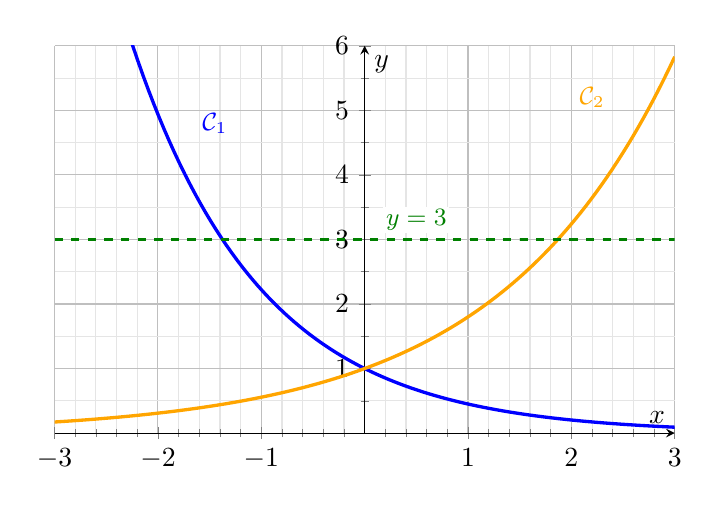
\begin{tikzpicture}
\begin{axis}[width=.78\textwidth,height=6.5cm,axis lines=middle,xmin=-3,xmax=3,ymin=0,ymax=6,
  xtick={-3,...,3},ytick={0,...,6},minor x tick num=4,minor y tick num=1,
  grid=both,major grid style={black!25},minor grid style={black!10},xlabel={$x$},ylabel={$y$}]
\addplot[Blue,very thick,samples=120,domain=-3:3]{0.45^x};
\addplot[Orange,very thick,samples=120,domain=-3:3]{1.8^x};
\addplot[Green,thick,dashed,domain=-3:3]{3};
\node[Blue,font=\small] at (axis cs:-1.45,4.8) {$\mathcal{C}_1$};
\node[Orange,font=\small] at (axis cs:2.2,5.2) {$\mathcal{C}_2$};
\node[Green,font=\small,fill=white,inner sep=1pt] at (axis cs:0.5,3.3) {$y=3$};
\end{axis}
\end{tikzpicture}
\end{center}
\begin{enumerate}
\item Which curve represents the function $f$? Justify your choice.
\item Solve the equation $f(x)=3$ graphically. Using a table of values on the calculator, give an approximate value of the solution to the nearest $0.01$.
\item Determine graphically the set of real numbers $x$ such that $f(x)\geqslant3$, then the set of real numbers $x$ such that $g(x)\geqslant3$.
\end{enumerate}
}{%
\begin{enumerate}
\item $1.8>1$, so $f$ is strictly increasing; $0<0.45<1$, so $g$ is strictly decreasing. The increasing curve $\mathcal{C}_2$ represents $f$ (and $\mathcal{C}_1$ represents $g$). Both curves pass through the point $(0;1)$.
\item The curve $\mathcal{C}_2$ meets the line $y=3$ at a point whose $x$-coordinate reads close to $1.9$. With the calculator: $1.8^{1.86}\approx2.984$ and $1.8^{1.87}\approx3.002$, so the solution lies between $1.86$ and $1.87$; the value $1.87$ gives the image closest to $3$. The solution is $x\approx1.87$.
\item $f(x)\geqslant3$ when $\mathcal{C}_2$ is above the line $y=3$, that is for $x\geqslant1.87$ approximately: $[1.87;+\infty[$ (approximate value of the endpoint).

$g$ is decreasing and $\mathcal{C}_1$ meets the line $y=3$ at an abscissa close to $-1.4$ (calculator: $0.45^{-1.38}\approx3.010$ and $0.45^{-1.37}\approx2.986$, so $x\approx-1.38$). Hence $g(x)\geqslant3$ for $x\leqslant-1.38$ approximately: $]-\infty;-1.38]$ (approximate value of the endpoint).
\end{enumerate}
}{5}

\DefExo{12}{Inequalities with the same base}{%
Solve the following inequalities on $\mathbb{R}$.
\begin{enumerate}[label=\alph*.]
\item $0.7^x\leqslant0.7^{-1}$
\item $2.5^{x+1}>2.5^4$
\item $0.5^x\geqslant0.25$
\end{enumerate}
}{%
\begin{enumerate}[label=\alph*.]
\item $0<0.7<1$: the function $x\mapsto0.7^x$ is strictly decreasing, so it reverses the order. Hence $0.7^x\leqslant0.7^{-1}\iff x\geqslant-1$. Solution set: $[-1;+\infty[$.
\item $2.5>1$: the function $x\mapsto2.5^x$ is strictly increasing, so it preserves the order. Hence $2.5^{x+1}>2.5^4\iff x+1>4\iff x>3$. Solution set: $]3;+\infty[$.
\item $0.25=0.5^2$, so the inequality reads $0.5^x\geqslant0.5^2$. Since $x\mapsto0.5^x$ is strictly decreasing: $x\leqslant2$. Solution set: $]-\infty;2]$.
\end{enumerate}
}{3}

\DefExo{13}{Model with $f(t)=ka^t$ and compute}{%
Just after an injection, the concentration of a drug in a patient's blood is $80$~mg/L. This concentration then decreases by $15\,\%$ every hour. This is an exponential decay.

It is modelled by a function $C$ of the time $t$, in hours, such that $C(t)=ka^t$.
\begin{enumerate}
\item Determine the constants $k$ and $a$.
\item Calculate the concentration after $3$~h~$30$~min, to the nearest $0.1$~mg/L.
\item The doctor plans a new injection as soon as the concentration drops below $50$~mg/L. Is this already the case after $3$~h~$30$~min? Answer in a sentence.
\end{enumerate}
}{%
\begin{enumerate}
\item $C(0)=k\times a^0=k$, and $C(0)=80$, so $k=80$. A $15\,\%$ decrease per hour corresponds to the multiplier $1-\dfrac{15}{100}=0.85$, so $a=0.85$ and $C(t)=80\times0.85^t$.
\item $3$~h~$30$~min $=3.5$~h. $C(3.5)=80\times0.85^{3.5}\approx45.3$~mg/L.
\item $45.3<50$: after $3$~h~$30$~min the concentration has already dropped below $50$~mg/L, so the new injection is due (in fact $C(3)\approx49.1$~mg/L, so the concentration is below this threshold from $3$~h onwards).
\end{enumerate}
}{4}

\DefExo{14}{Average rate of two successive changes}{%
\begin{enumerate}
\item The price of a digital currency rises by $125\,\%$ one year, then falls by $36\,\%$ the following year. What is the average annual rate of change over these two years?
\item The price of a raw material rises by $80\,\%$ one month, then falls by $55\,\%$ the following month. What is the average monthly rate of change?
\item A student claims that, in question 2, the average rate is $\dfrac{80-55}{2}=12.5\,\%$. Explain in a sentence why this is wrong.
\end{enumerate}
}{%
\begin{enumerate}
\item The multipliers are $1+\dfrac{125}{100}=2.25$ and $1-\dfrac{36}{100}=0.64$. The overall multiplier is $2.25\times0.64=1.44$. The average annual multiplier $q$ satisfies $q^2=1.44$, so $q=\sqrt{1.44}=1.2$: an average annual rise of $20\,\%$.
\item The multipliers are $1.8$ and $0.45$; the overall multiplier is $1.8\times0.45=0.81$. The average multiplier is $\sqrt{0.81}=0.9$, that is an average monthly fall of $10\,\%$.
\item Successive changes combine by multiplying the multipliers, not by adding the rates: the $55\,\%$ fall applies to a price that has already risen. Over the two months the price is multiplied by $0.81$ (an overall fall of $19\,\%$), which corresponds to an average fall of $10\,\%$ per month, not a rise of $12.5\,\%$.
\end{enumerate}
}{5}
